% Created 2024-06-11 Τρι 13:38
% Intended LaTeX compiler: pdflatex
\documentclass[11pt]{article}
\usepackage[utf8]{inputenc}
\usepackage[T1]{fontenc}
\usepackage{graphicx}
\usepackage{longtable}
\usepackage{wrapfig}
\usepackage{rotating}
\usepackage[normalem]{ulem}
\usepackage{amsmath}
\usepackage{amssymb}
\usepackage{capt-of}
\usepackage{hyperref}
\usepackage{booktabs}
\usepackage{import}
\usepackage[LGR, T1]{fontenc}
\usepackage[greek, english, american]{babel}
\usepackage{alphabeta}
\usepackage{esint}
\usepackage{mathtools}
\usepackage{esdiff}
\usepackage{makeidx}
\usepackage[acronym]{glossaries}
\usepackage{newfloat}
\usepackage{minted}
\usepackage[a4paper, margin=3cm]{geometry}
\usepackage{chemfig}
\usepackage{svg}
\author{Βιδιάνος Γιαννίτσης}
\date{\today}
\title{Σύγκριση δεδομένων HPLC και COD}
\hypersetup{
 pdfauthor={Βιδιάνος Γιαννίτσης},
 pdftitle={Σύγκριση δεδομένων HPLC και COD},
 pdfkeywords={},
 pdfsubject={},
 pdfcreator={Emacs 29.3 (Org mode 9.6.15)}, 
 pdflang={English}}
\makeatletter
\newcommand{\citeprocitem}[2]{\hyper@linkstart{cite}{citeproc_bib_item_#1}#2\hyper@linkend}
\makeatother

\usepackage[notquote]{hanging}
\begin{document}

\maketitle
\tableofcontents

\begin{abstract}
Η ανάλυση COD είναι μία ανάλυση που μετράει την συνολική οργανική ύλη μίας ένωσης με βάση το πόσο οξυγόνο θέλει για να οξειδωθεί πλήρως. Η ανάλυση της HPLC μετράει την συγκέντρωση για συγκεκριμένα χημικά είδη. Συγκρίνοντας τα δεδομένα των δύο αναλύσεων μπορούμε να δούμε πόση από την οργανική ύλη που μπορεί να υπάρχει μετράει όντως η HPLC και πόση είναι άλλες, άγνωστες ενώσεις. Βέβαια, λόγω των μεγάλων αραιώσεων που απαιτούνται για να μετρηθεί το COD, πολλές φορές δεν έχει ικανοποιητική ακρίβεια, το οποίο μπορεί να δημιουργήσει προβλήματα στην σύγκριση αυτή. Ένα άλλο ενδιαφέρον που έχει μία τέτοια ανάλυση είναι πως μας επιτρέπει να δούμε πόσο από το συνολικό sCOD στο τέλος της διεργασίας είναι πτητικά λιπαρά οξέα (VFAs), ένα κριτήριο του πόσο καλό acidification έγινε στον αντιδραστήρα. Το αρχείο αυτό αποτελεί ένα literate document που επεξηγεί την διαδικασία αυτή αναλυτικά και δείχνει τα αποτελέσματα της, ενώ μπορεί να κάνει tangle τον κώδικα που αναφέρεται στα κατάλληλα scripts ή να τον κάνει weave σε ένα pdf. Αξίζει να αναφερθεί πως γίνεται έντονη named code blocks τα οποία βοηθάνε στο να τρέξουμε πολλές φορές το ίδιο code block με βάση του noweb syntax που προσφέρει το org-mode. Καθώς το όνομα του code block δεν γίνεται weaved, θα υπάρχει με bold το όνομα πριν ακριβώς από κάθε code block, ώστε να μπορεί να κατανοηθεί και πότε κάποιο γίνεται inserted σε άλλα.
\end{abstract}

\section{Dependencies}
\label{sec:org7b57b41}
Καθώς το project αυτό είναι δομημένο με το πακέτο DrWatson της Julia για να κάνει facilitate reproducibility, πρέπει σε όλα τα αρχεία να υπάρχουν τα lines που ενεργοποιούν το DrWatson και πηγαίνουν στο κατάλληλο project. Έπειτα, είναι επίσης απαραίτητο να κάνουμε include κάποια functions για την ανάλυση των δεδομένων το οποίο υπάρχει στο src directory και είναι amply documented εκεί.

\textbf{dependencies}
\begin{minted}[breaklines=true,breakanywhere=true]{julia}
using DrWatson
@quickactivate "Masters_Thesis"
include(srcdir("cod_balance.jl"))
include(srcdir("filenames.jl"))
using CSV, DataFrames
using StatsPlots
\end{minted}

\section{Data Reading and Processing}
\label{sec:org3a2f586}
Αρχικά πρέπει να διαβάσουμε τα δεδομένα των δύο αναλύσεων από τα CSV τους. Θα υποθέσουμε πως τα δεδομένα της HPLC είναι ήδη επεξεργασμένα και απλώς θα διαβάσουμε τα csv με τις συγκεντρώσεις. Για να παραχθούν αυτά, μπορούμε να κάνουμε refer στο αντίστοιχο \href{./hplc\_analysis\_notebook.org}{notebook}, στο οποίο εξηγείται και περισσότερο τι πειράματα έχουν γίνει και πως τα διαχειριζόμαστε. To COD είναι έτοιμο στην processed μορφή του για τα πειράματα στις 10 και 28 Νοεμβρίου ενώ για το αρχικό πείραμα της κινητικής, υπάρχει μόνο ένας πίνακας με διάφορες πληροφορίες συμπεριλαμβανομένου της απορρόφησης του COD, οπότε απαιτείται ένα παραπάνω processing step εκεί.

Αρχικά θα γραφεί το code block που κάνει το generic processing των δεδομένων και βασίζεται στο variable date και μετά θα γραφούν τα blocks που το τρέχουν για τις διαφορετικές ημερομηνίες. Εκτός από να διαβάσουμε τα δεδομένα της HPLC, πρέπει να κάνουμε extract μόνο την πρώτη και την τελευταία μέρα επειδή αυτές υπάρχουν στο COD. Έπειτα, για να έχουμε συγκρίσιμα μεγέθη, υπολογίζουμε το COD-eq κάθε ένωσης και κάνουμε τις μετατροπές. Αυτό φαίνεται παρακάτω. 

\textbf{cod\textsubscript{data}\textsubscript{extraction}}
\begin{minted}[breaklines=true,breakanywhere=true]{julia}

mix_amount = ["0", "1", "2", "4", "8"]
df0_conc = CSV.read(get_conc_csv(date, mix_amount[1]), DataFrame)
df1_conc = CSV.read(get_conc_csv(date, mix_amount[2]), DataFrame)
df2_conc = CSV.read(get_conc_csv(date, mix_amount[3]), DataFrame)
df4_conc = CSV.read(get_conc_csv(date, mix_amount[4]), DataFrame)
df8_conc = CSV.read(get_conc_csv(date, mix_amount[5]), DataFrame)

cod_meas = CSV.read(get_cod_csv(date), DataFrame)

df0_conc0 = Vector(df0_conc[1, 2:8])
df1_conc0 = Vector(df1_conc[1, 2:8])
df2_conc0 = Vector(df2_conc[1, 2:8])
df4_conc0 = Vector(df4_conc[1, 2:8])
df8_conc0 = Vector(df8_conc[1, 2:8])

df0_conc72 = Vector(df0_conc[4, 2:8])
df1_conc72 = Vector(df1_conc[4, 2:8])
df2_conc72 = Vector(df2_conc[4, 2:8])
df4_conc72 = Vector(df4_conc[4, 2:8])
df8_conc72 = Vector(df8_conc[4, 2:8])

cod_yields = [cod_sucrose(), cod_glucose(), cod_fructose(), cod_acetate(),
              cod_propionate(), cod_lactate(), cod_ethanol()]

df0_cod0 = df0_conc0.*cod_yields
df1_cod0 = df1_conc0.*cod_yields
df2_cod0 = df2_conc0.*cod_yields
df4_cod0 = df4_conc0.*cod_yields
df8_cod0 = df8_conc0.*cod_yields

df0_cod0_sum = sum(df0_cod0)
df1_cod0_sum = sum(df1_cod0)
df2_cod0_sum = sum(df2_cod0)
df4_cod0_sum = sum(df4_cod0)
df8_cod0_sum = sum(df8_cod0)

cod0_theor = [df0_cod0_sum, df1_cod0_sum, df2_cod0_sum, df4_cod0_sum, df8_cod0_sum]
cod0_meas = cod_meas.COD_0./1000
cod0_error = cod0_meas - cod0_theor

df0_cod72 = df0_conc72.*cod_yields
df1_cod72 = df1_conc72.*cod_yields
df2_cod72 = df2_conc72.*cod_yields
df4_cod72 = df4_conc72.*cod_yields
df8_cod72 = df8_conc72.*cod_yields

df0_VFA_cod = df0_cod72[4:7]
df1_VFA_cod = df1_cod72[4:7]
df2_VFA_cod = df2_cod72[4:7]
df4_VFA_cod = df4_cod72[4:7]
df8_VFA_cod = df8_cod72[4:7]
VFA_vec = [hcat(df0_VFA_cod, df1_VFA_cod, df2_VFA_cod, df4_VFA_cod, df8_VFA_cod)[i, :] for i in 1:4]

df0_cod72_sum = sum(df0_cod72)
df1_cod72_sum = sum(df1_cod72)
df2_cod72_sum = sum(df2_cod72)
df4_cod72_sum = sum(df4_cod72)
df8_cod72_sum = sum(df8_cod72)

cod72_theor = [df0_cod72_sum, df1_cod72_sum, df2_cod72_sum, df4_cod72_sum, df8_cod72_sum]
cod72_meas = cod_meas.COD_72./1000
cod72_error = cod72_meas - cod72_theor

\end{minted}

\section{Acidification Rate}
\label{sec:orgcb787cc}
Όπως αναφέρθηκε παραπάνω, ένα ακόμη χρήσιμο κριτήριο που μπορεί να γίνει κάνοντας convert τα αποτελέσματα της HPLC στο COD-eq τους είναι να δούμε πόσο καλό acidification έχει γίνει συγκρίνοντας ολικό διαλυτό COD με διαλυτό COD που οφείλεται στα προιόντα της οξεογένεσης. Για αυτά, θα χρησιμοποιηθεί παρακάτω ο όρος VFAs (volatile fatty acids) αλλά κατά σύμβαση θα συμπεριληφθεί σε αυτά και η αιθανόλη καθώς παρότι δεν είναι VFA είναι ένα από τα βασικά προιόντα μίας οξεογένεσης (ειδικά αν αυτή γίνεται σε χαμηλό pH).

\begin{minted}[breaklines=true,breakanywhere=true]{julia}

date = "10_11"
<<cod_data_extraction>>
df0_35_tVFA = sum(df0_VFA_cod)
df1_35_tVFA = sum(df1_VFA_cod)
df2_35_tVFA = sum(df2_VFA_cod)
df4_35_tVFA = sum(df4_VFA_cod)
df8_35_tVFA = sum(df8_VFA_cod)

tVFA_35 = [df0_35_tVFA, df1_35_tVFA, df2_35_tVFA, df4_35_tVFA, df8_35_tVFA]
acidification_35 = tVFA_35./cod72_meas

date = "28_11"
<<cod_data_extraction>>
df0_40_tVFA = sum(df0_VFA_cod)
df1_40_tVFA = sum(df1_VFA_cod)
df2_40_tVFA = sum(df2_VFA_cod)
df4_40_tVFA = sum(df4_VFA_cod)
df8_40_tVFA = sum(df8_VFA_cod)

tVFA_40 = [df0_40_tVFA, df1_40_tVFA, df2_40_tVFA, df4_40_tVFA, df8_40_tVFA]
acidification_40 = tVFA_40./cod72_meas

date = "23_10"
df1_45_conc = CSV.read(get_conc_csv(date, "1"), DataFrame)
df1_45_conc = df1_45_conc[1:19, 2:8]

df2_45_conc = CSV.read(get_conc_csv(date, "2"), DataFrame)
df2_45_conc = df2_45_conc[1:15, 2:8]

cod_yields = [cod_sucrose(), cod_glucose(), cod_fructose(), cod_acetate(),
              cod_propionate(), cod_lactate(), cod_ethanol()]
df1_45_tVFA = [sum(Vector(df1_45_conc[i, 4:7]).*cod_yields[4:7]) for i in 1:19]
df2_45_tVFA = [sum(Vector(df2_45_conc[i, 4:7]).*cod_yields[4:7]) for i in 1:15]

cod_1_meas = process_cod_data("1", date; dilution = 50)./1000
cod_2_meas = process_cod_data("2", date; dilution = 50)./1000

acidification_45 = [0, 0, mean([df1_45_tVFA[15]/cod_1_meas[15], df2_45_tVFA[11]/cod_2_meas[11]]), 0, 0]

acid_plot = groupedbar([0, 1, 2, 3, 4], [acidification_35 acidification_40 acidification_45],
                       label = ["35 C" "40 C" "45 C"], xlabel = "Amount of mix (ml)",
                       ylabel = "tVFAs (gCOD-eq/L)/sCOD (g/L)",
                       title = "Acidification Rate", xticks = (0:4, mix_amount),
                       legend = :bottom)
savefig(acid_plot, plotsdir("35_40_45_comp", "acidification_comp.png"))

\end{minted}

\begin{center}
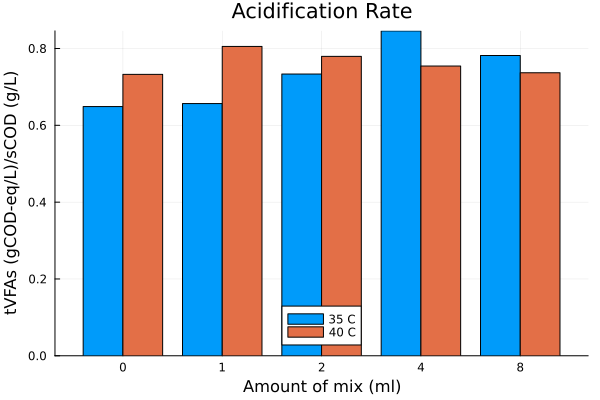
\includegraphics[width=.9\linewidth]{../plots/35_40_comp/acidification_comp.png}
\end{center}

\section{Plotting}
\label{sec:org75df20b}
Με αυτά τα δεδομένα, μπορούμε να κάνουμε κάποια χρήσιμα διαγράμματα. Θα κάνουμε 2 κατηγορίες διαγραμμάτων.

Η πρώτη θα είναι συγκριτικά διαγράμματα των αποτελεσμάτων της ανάλυσης COD και του υπολογισμένου COD από την HPLC ενώ η δεύτερη θα είναι κάποια stacked bar plots που θα δείχνουν τις τελικές συγκεντρώσεις όλων των προιόντων σε COD-eq. Το πρώτο έχει τον συγκριτικό σκοπό του να δούμε πόσο από το διαλυτό COD είναι οι 7 ενώσεις που μετράμε στην HPLC ενώ το δεύτερο είναι συνοδευτικό του παραπάνω για να κρίνουμε ποιο δείγμα παρήγαγε τα περισσότερα οξέα. Σε άλλο αρχείο έχει γίνει το αντίστοιχο plot και σε συγκέντρωση αντί για COD-eq.

\textbf{cod\textsubscript{plots}}
\begin{minted}[breaklines=true,breakanywhere=true]{julia}

label = ["COD Measurement" "HPLC Measurement"]
plot_type = "comparison"

cod0_comp_plot = groupedbar([0, 1, 2, 3, 4], [cod0_meas cod0_theor],
                       label = label, xlabel = "Amount of mix (ml)",
                       ylabel = "COD (g/l)", legend =:bottom,
                       title = "COD comparison t=0",
                       xticks = (0:4, mix_amount))
savefig(cod0_comp_plot, get_plot_name("cod_0", date, plot_type))

cod72_comp_plot = groupedbar([0, 1, 2, 3, 4], [cod72_meas cod72_theor],
                       label = label, xlabel = "Amount of mix (ml)",
                       ylabel = "COD (g/l)", legend =:bottom,
                       title = "COD comparison t=72 h",
                       xticks = (0:4, mix_amount))
savefig(cod72_comp_plot, get_plot_name("cod_72", date, plot_type))

cod_comp_plot = plot(cod0_comp_plot, cod72_comp_plot, layout = (2,1), size = (900, 600))
savefig(cod_comp_plot, get_plot_name("cod", date, plot_type))

plot_type = "bar"
cod0_plot = bar([0, 1, 2, 3, 4], cod0_meas,
                xlabel = "Amount of mix (ml)",
                ylabel = "COD (g/l)", legend = false,
                title = "COD @t=0",
                xticks = (0:4, mix_amount))
savefig(cod0_comp_plot, get_plot_name("cod_0", date, plot_type))

cod72_plot = bar([0, 1, 2, 3, 4], cod72_meas,
                 xlabel = "Amount of mix (ml)",
                 ylabel = "COD (g/l)", legend = false,
                 title = "COD @t=72 h",
                 xticks = (0:4, mix_amount), fc = "#E36F47")
savefig(cod72_comp_plot, get_plot_name("cod_72", date, plot_type))

cod_plot = plot(cod0_plot, cod72_plot, layout = (2,1), size = (900, 600))
savefig(cod_plot, get_plot_name("cod", date, plot_type))

cod_groupedbar = groupedbar([0, 1, 2, 3, 4], [cod0_meas cod72_meas],
                            xlabel = "Amount of mix (mL)",
                            ylabel = "COD (g/l)", label = ["0h" "72h"],
                            xticks = (0:4, mix_amount),
                            title = "COD during Hydrolysis")
savefig(cod_groupedbar, get_plot_name("cod", date, "groupedbar"))

vfa_plot = groupedbar([0, 1, 2, 3, 4],
                      [VFA_vec[1] VFA_vec[2] VFA_vec[3] VFA_vec[4]],
                      bar_position = :stack, xticks = (0:4, mix_amount),
                      label = ["Lactate" "Acetate" "Propionate" "Ethanol"],
                      xlabel = "Amount of mix (ml)", ylabel = "VFAs (g COD-eq/L)",
                      title = "VFAs Produced during Fermentation",
                      legend = :outerright)
savefig(vfa_plot, get_plot_name("vfa_cod", date, "stackedbar"))
\end{minted}

\section{Αποτελέσματα για το πείραμα 10/11}
\label{sec:org18b2cb3}
Έχοντας τα παραπάνω code blocks, μπορούμε ορίζοντας το date και τρέχοντας τα να παράγουμε τα απαιτούμενα plots. Το συγκεντρωτικό plot φαίνεται παρακάτω. Επίσης, αυτό ακριβώς είναι και αυτό που θέλουμε να γίνει tangled, μόλις φυσικά κάνουμε tangle τα dependencies.

\begin{minted}[breaklines=true,breakanywhere=true]{julia}
<<dependencies>>
\end{minted}

\begin{minted}[breaklines=true,breakanywhere=true]{julia}

date = "10_11"
<<cod_data_extraction>>
<<cod_plots>>

\end{minted}

\begin{figure}[htbp]
\centering
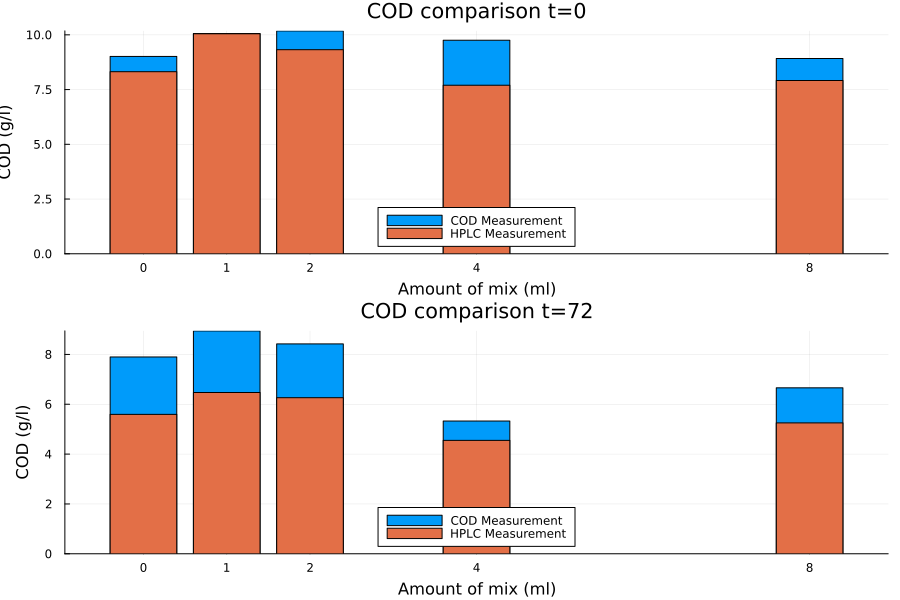
\includegraphics[width=.9\linewidth]{/home/vidianos/Documents/9o_εξάμηνο/Masters_Thesis/plots/10_11/cod_comparison_10_11.png}
\caption{Σύγκριση της μέτρησης COD άμεσα ή μέσω της HPLC - Πείραμα 10/11}
\end{figure}

\begin{center}
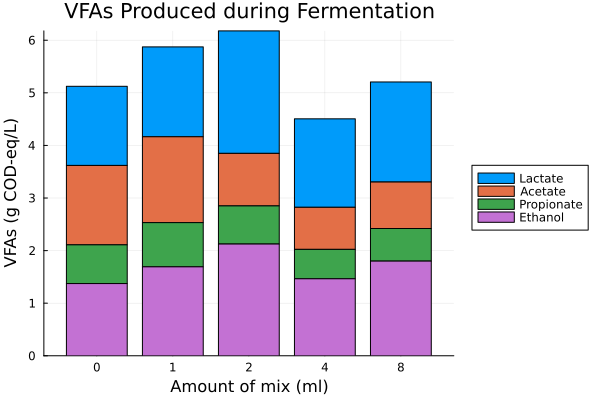
\includegraphics[width=.9\linewidth]{../plots/10_11/vfa_cod_stackedbar_10_11.png}
\end{center}

\begin{center}
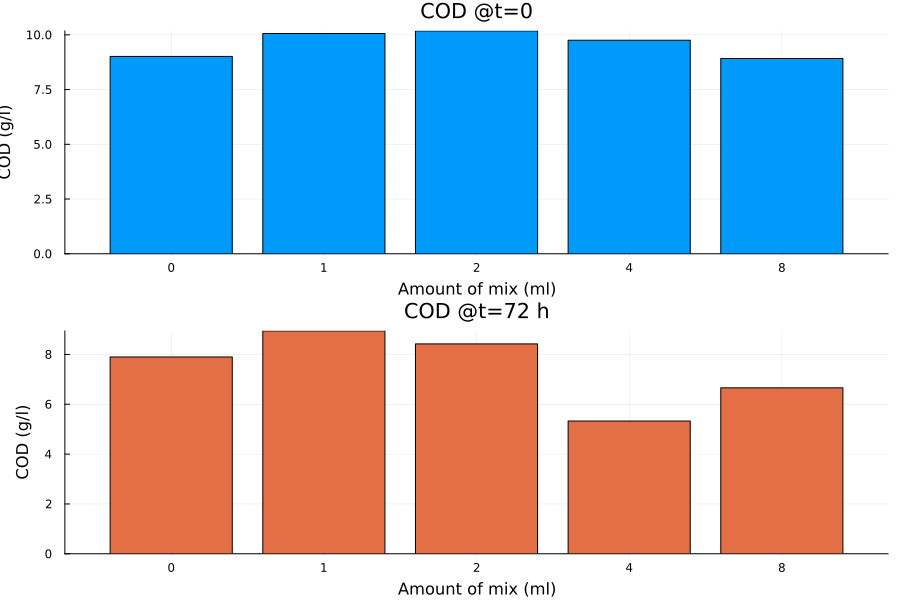
\includegraphics[width=.9\linewidth]{../plots/10_11/cod_bar_10_11.png}
\end{center}

\section{Αποτελέσματα για το πείραμα 28/11}
\label{sec:org90cccc4}
Ομοίως, μπορούμε αλλάζοντας το date να τρέξουμε και το πείραμα της 28/11 χωρίς καμία πρακτική αλλαγή στον κώδικα.

\begin{minted}[breaklines=true,breakanywhere=true]{julia}
<<dependencies>>
\end{minted}

\begin{minted}[breaklines=true,breakanywhere=true]{julia}

date = "28_11"
<<cod_data_extraction>>
<<cod_plots>>

\end{minted}

\begin{figure}[htbp]
\centering
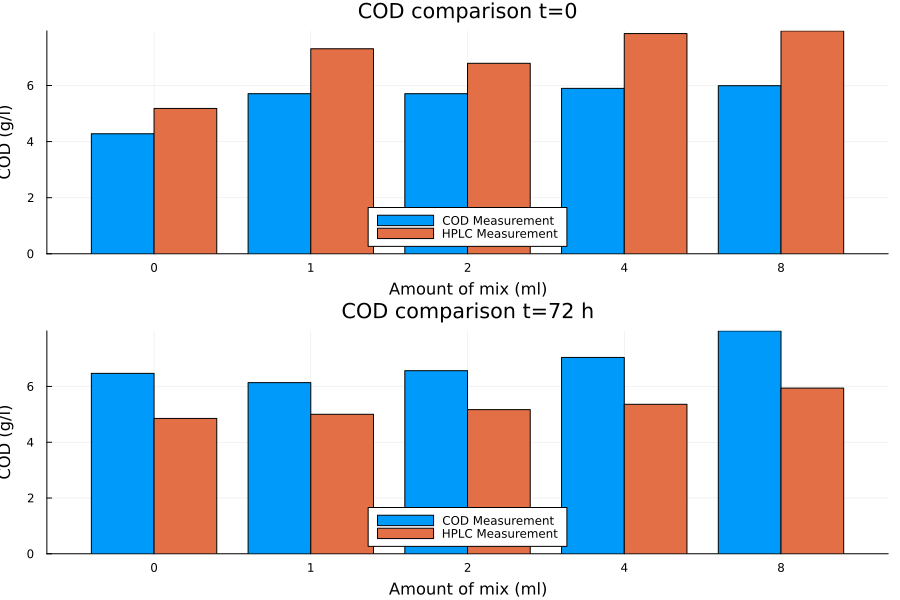
\includegraphics[width=.9\linewidth]{/home/vidianos/Documents/9o_εξάμηνο/Masters_Thesis/plots/28_11/cod_comparison_28_11.png}
\caption{Σύγκριση της μέτρησης COD άμεσα ή μέσω της HPLC - Πείραμα 28/11}
\end{figure}

\begin{center}
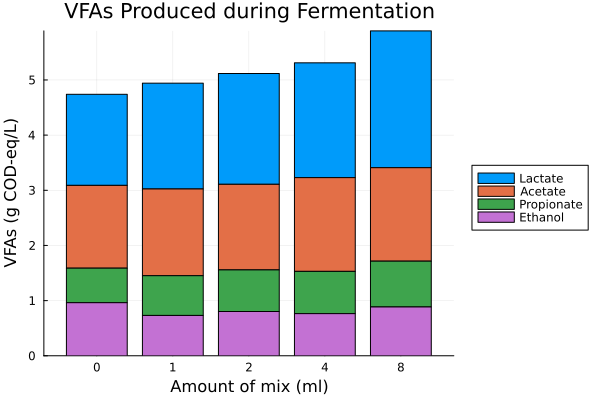
\includegraphics[width=.9\linewidth]{../plots/28_11/vfa_cod_stackedbar_28_11.png}
\end{center}

\begin{center}
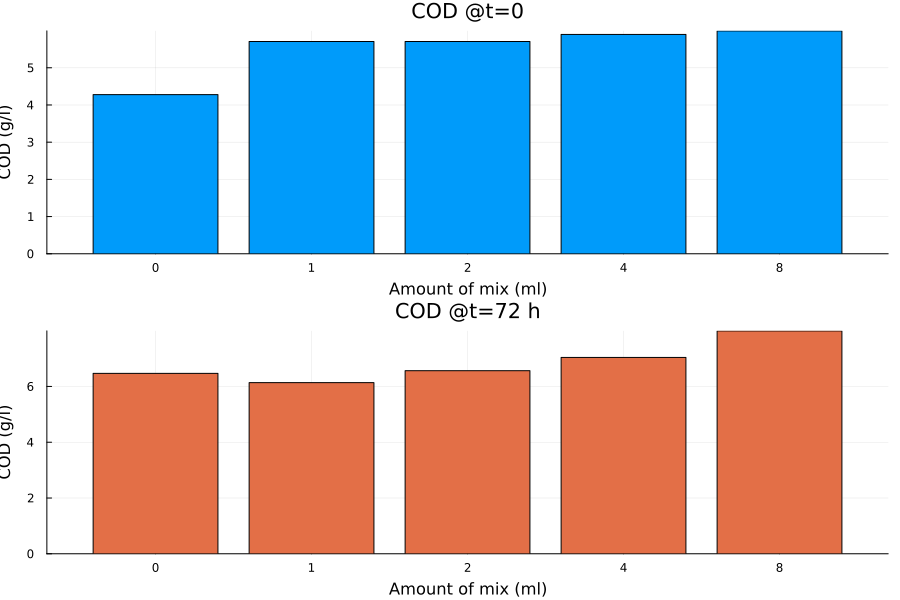
\includegraphics[width=.9\linewidth]{../plots/28_11/cod_bar_28_11.png}
\end{center}

\section{Πείραμα 23/10}
\label{sec:orgbf738f4}
Στο πείραμα αυτό υπήρχε καθημερινή μέτρηση του COD, εκτός από την τελευταία μέρα που ήταν μετά το σαββατοκύριακο οπότε έχει νόημα να γίνει σύγκριση σε όλα τα διαθέσιμα σημεία.

\subsection{HPLC Data}
\label{sec:org3c6643d}
Αρχικά διαβάζουμε τα δεδομένα της HPLC και κάνουμε τις μετατροπές σε COD-eq.

\textbf{hplc\textsubscript{data}\textsubscript{processing}\textsubscript{23}\textsubscript{10}}
\begin{minted}[breaklines=true,breakanywhere=true]{julia}

date = "23_10"
df1_conc = CSV.read(get_conc_csv(date, "1"), DataFrame)
t1 = df1_conc[1:19, 1]
df1_conc = df1_conc[1:19, 2:8]
df2_conc = CSV.read(get_conc_csv(date, "2"), DataFrame)
t2 = df2_conc[1:15, 1]
df2_conc = df2_conc[1:15, 2:8]

cod_yields = [cod_sucrose(), cod_glucose(), cod_fructose(), cod_acetate(),
              cod_propionate(), cod_lactate(), cod_ethanol()]

cod_1_theor = [sum(Vector(df1_conc[i, :]).*cod_yields) for i in 1:19]
cod_2_theor = [sum(Vector(df2_conc[i, :]).*cod_yields) for i in 1:15]

\end{minted}

\subsection{COD Data}
\label{sec:orga1f787e}
Έπειτα, κάνουμε την επεξεργασία του COD data, το οποίο για αυτό το πείραμα δεν υπήρχε διαθέσιμο σε συγκέντρωση αλλά μόνο σε απορρόφηση. Όμως ο κώδικας είναι πολύ compact λόγω του helper function \texttt{process\_cod\_data} που κάνει την μετατροπή μόνο του.

\textbf{cod\textsubscript{data}\textsubscript{processing}\textsubscript{23}\textsubscript{10}}
\begin{minted}[breaklines=true,breakanywhere=true]{julia}

cod_1_meas = process_cod_data("1", date; dilution = 50)./1000
cod_1_error = cod_1_meas - cod_1_theor
cod_2_meas = process_cod_data("2", date; dilution = 50)./1000
cod_2_error = cod_2_meas - cod_2_theor

\end{minted}

\subsection{Plotting}
\label{sec:org3f7470a}
Τέλος, μπορούν να γίνουν τα plots για αυτό το πείραμα που λόγω του πλήθους των στοιχείων έχει νόημα μόνο να είναι σε scatter plot.

\textbf{cod\textsubscript{balance}\textsubscript{plots}\textsubscript{23}\textsubscript{10}}
\begin{minted}[breaklines=true,breakanywhere=true]{julia}

label = ["COD Measurement" "HPLC Measurement"]
plot_type = "comparison"

cod_1_plot = scatter(t1, [cod_1_meas cod_1_theor], label=label,
                 xlabel = "Time (h)", ylabel = "COD (g/l)",
                 title = "Sample 1", markersize = 6)
savefig(cod_1_plot, get_plot_name("cod_1", date, plot_type))

cod_2_plot = scatter(t2, [cod_2_meas cod_2_theor], label=label,
                 xlabel = "Time (h)", ylabel = "COD (g/l)",
                 title = "Sample 2", markersize = 6)
savefig(cod_2_plot, get_plot_name("cod_2", date, plot_type))

cod_plot = plot(cod_1_plot, cod_2_plot, layout = (2,1), size = (900, 600))
savefig(cod_plot, get_plot_name("cod", date, plot_type))

cod_meas_plot_1 = scatter(t1, cod_1_meas, xlabel = "Time (h)", ylabel = "COD (g/l)",
                          title = "Sample 1", markersize = 4,
                          markercolor = "#009AFA", legend = false)
plot!(t1, cod_1_meas, linecolor = "#009AFA")
cod_meas_plot_2 = scatter(t2, cod_2_meas, xlabel = "Time (h)", ylabel = "COD (g/l)",
                          title = "Sample 2", markersize = 4,
                          markercolor = "#E36F47", legend = false)
plot!(t2, cod_2_meas, linecolor = "#E36F47")
cod_meas_plot = plot(cod_meas_plot_1, cod_meas_plot_2, size = (900, 600), left_margin = 3Plots.mm, plot_title = "COD Measurements")
savefig(cod_meas_plot, get_plot_name("cod", date, "scatter"))
\end{minted}

\subsection{Τελικά code blocks}
\label{sec:org6db5a80}
Έπειτα, βάζουμε το τελικό code block που με χρήση του noweb syntax θα κάνει tangle στα script files.

\begin{minted}[breaklines=true,breakanywhere=true]{julia}
<<dependencies>>
\end{minted}

\begin{minted}[breaklines=true,breakanywhere=true]{julia}

<<hplc_data_processing_23_10>>
<<cod_data_processing_23_10>>
<<cod_balance_plots_23_10>>

\end{minted}

\begin{figure}[htbp]
\centering
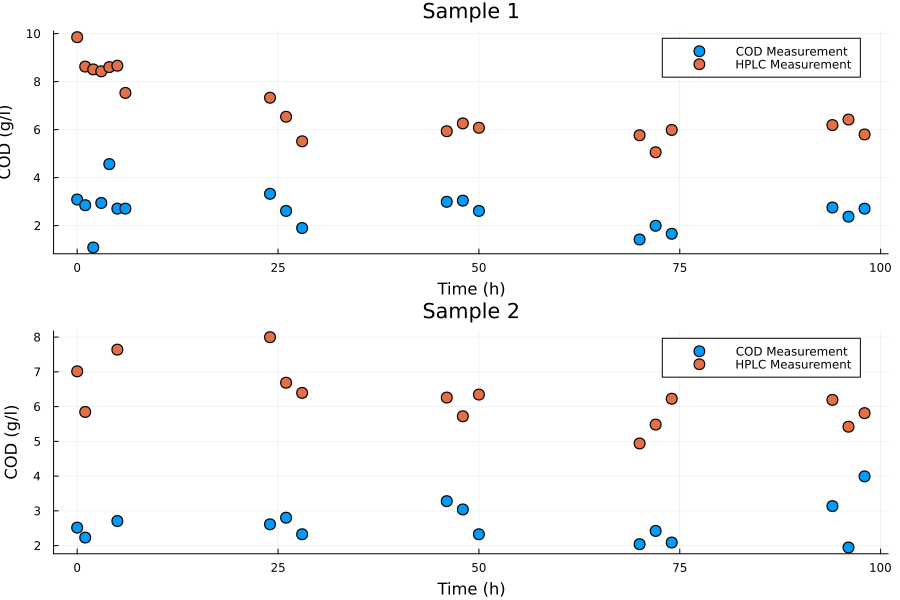
\includegraphics[width=.9\linewidth]{/home/vidianos/Documents/9o_εξάμηνο/Masters_Thesis/plots/23_10/cod_comparison_23_10.png}
\caption{Σύγκριση της μέτρησης COD άμεσα ή μέσω της HPLC - Πείραμα 23/10}
\end{figure}

\section{Πείραμα 06\textsubscript{06}}
\label{sec:org6326b4b}
Στο πείραμα αυτό έγιναν οι αναλύσεις για το αρχικό FW, τα υδρολύματα της ORCA και τέλος του υδρολύματος που χρησιμοποιήθηκε ως feedstock για την αναερόβια χώνευση.
\subsection{HPLC Data}
\label{sec:orgcd08d27}
Αρχικά διαβάζουμε τα δεδομένα της HPLC και κάνουμε τις μετατροπές σε COD-eq.

\textbf{hplc\textsubscript{data}\textsubscript{processing}\textsubscript{06}\textsubscript{06}}
\begin{minted}[breaklines=true,breakanywhere=true]{julia}

date = "06_06"
df0606_conc = CSV.read(get_conc_csv(date, "1"), DataFrame)
df1_conc = df0606_conc[:, 2:end]
fw_df = df1_conc[1, :]
fw_conc = Vector(fw_df)

orca_df = df0606_conc[2:3, :]
orca_conc = Matrix(orca_df[:, 2:end])

hydro_40 = df0606_conc[4:11, :]

cod_yields = [cod_sucrose(), cod_glucose(), cod_fructose(), cod_acetate(),
              cod_propionate(), cod_lactate(), cod_ethanol()]

cod_1_theor = [sum(Vector(df1_conc[i, :]).*cod_yields) for i in 1:11]

\end{minted}

\begin{verbatim}
15-element Vector{Float64}:
 7.015000272531603
 5.846938417433187
 7.6399174100207325
 7.997976681370974
 6.6871703605535835
 6.395296146167445
 6.2604839683030225
 5.72184891837552
 6.3462461803153385
 4.939608588161173
 5.482878203834697
 6.226055413739973
 6.19398460285115
 5.421508167019161
 5.811939563034854
\end{verbatim}

\subsection{COD Data}
\label{sec:org95bc10d}
Έπειτα, κάνουμε την επεξεργασία του COD data, το οποίο για αυτό το πείραμα δεν υπήρχε διαθέσιμο σε συγκέντρωση αλλά μόνο σε απορρόφηση. Όμως ο κώδικας είναι πολύ compact λόγω του helper function \texttt{process\_cod\_data} που κάνει την μετατροπή μόνο του.

\textbf{cod\textsubscript{data}\textsubscript{processing}\textsubscript{23}\textsubscript{10}}
\begin{minted}[breaklines=true,breakanywhere=true]{julia}

cod_1_meas = process_cod_data("1", date; dilution = 50)./1000
cod_1_error = cod_1_meas - cod_1_theor
cod_2_meas = process_cod_data("2", date; dilution = 50)./1000
cod_2_error = cod_2_meas - cod_2_theor

\end{minted}

\subsection{Plotting}
\label{sec:org50e6bcd}
Τέλος, μπορούν να γίνουν τα plots για αυτό το πείραμα που λόγω του πλήθους των στοιχείων έχει νόημα μόνο να είναι σε scatter plot.

\textbf{cod\textsubscript{balance}\textsubscript{plots}\textsubscript{23}\textsubscript{10}}
\begin{minted}[breaklines=true,breakanywhere=true]{julia}

label = ["COD Measurement" "HPLC Measurement"]
plot_type = "comparison"

cod_1_plot = scatter(t1, [cod_1_meas cod_1_theor], label=label,
                 xlabel = "Time (h)", ylabel = "COD (g/l)",
                 title = "Sample 1", markersize = 6)
savefig(cod_1_plot, get_plot_name("cod_1", date, plot_type))

cod_2_plot = scatter(t2, [cod_2_meas cod_2_theor], label=label,
                 xlabel = "Time (h)", ylabel = "COD (g/l)",
                 title = "Sample 2", markersize = 6)
savefig(cod_2_plot, get_plot_name("cod_2", date, plot_type))

cod_plot = plot(cod_1_plot, cod_2_plot, layout = (2,1), size = (900, 600))
savefig(cod_plot, get_plot_name("cod", date, plot_type))

cod_meas_plot_1 = scatter(t1, cod_1_meas, xlabel = "Time (h)", ylabel = "COD (g/l)",
                          title = "Sample 1", markersize = 4,
                          markercolor = "#009AFA", legend = false)
plot!(t1, cod_1_meas, linecolor = "#009AFA")
cod_meas_plot_2 = scatter(t2, cod_2_meas, xlabel = "Time (h)", ylabel = "COD (g/l)",
                          title = "Sample 2", markersize = 4,
                          markercolor = "#E36F47", legend = false)
plot!(t2, cod_2_meas, linecolor = "#E36F47")
cod_meas_plot = plot(cod_meas_plot_1, cod_meas_plot_2, size = (900, 600), left_margin = 3Plots.mm, plot_title = "COD Measurements")
savefig(cod_meas_plot, get_plot_name("cod", date, "scatter"))
\end{minted}

\subsection{Τελικά code blocks}
\label{sec:org063d8af}
Έπειτα, βάζουμε το τελικό code block που με χρήση του noweb syntax θα κάνει tangle στα script files.

\begin{minted}[breaklines=true,breakanywhere=true]{julia}
<<dependencies>>
\end{minted}

\begin{minted}[breaklines=true,breakanywhere=true]{julia}

<<hplc_data_processing_23_10>>
<<cod_data_processing_23_10>>
<<cod_balance_plots_23_10>>

\end{minted}

\begin{figure}[htbp]
\centering
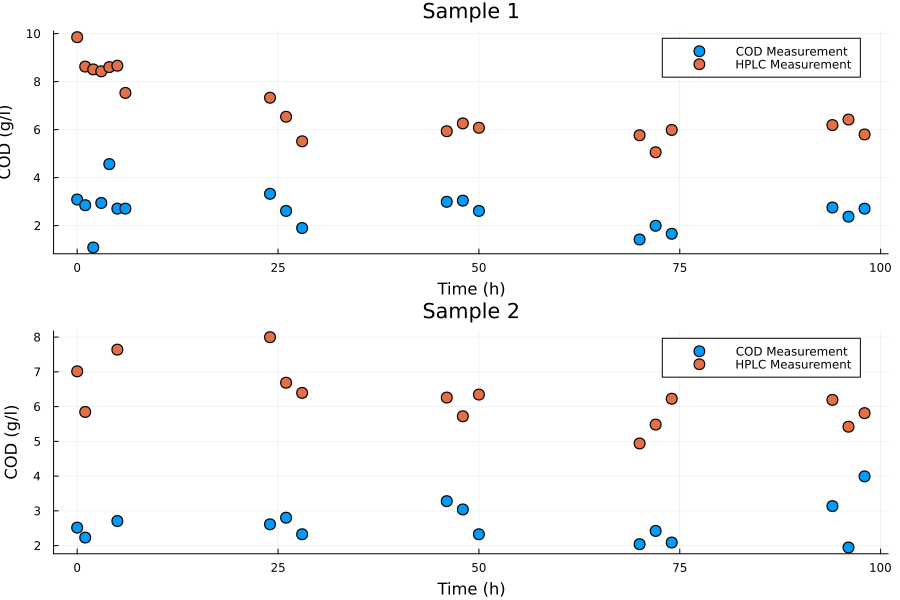
\includegraphics[width=.9\linewidth]{/home/vidianos/Documents/9o_εξάμηνο/Masters_Thesis/plots/23_10/cod_comparison_23_10.png}
\caption{Σύγκριση της μέτρησης COD άμεσα ή μέσω της HPLC - Πείραμα 23/10}
\end{figure}
\end{document}
